\documentclass[compress]{beamer}
\usepackage{ifthen,verbatim}

\title{Lessons learned in CSA07}
\author{Jim Pivarski, Alexei Safonov}
\institute{Texas A\&M University}
\date{ 2 November, 2007}

\newcommand{\isnote}{}
\xdefinecolor{lightyellow}{rgb}{1.,1.,0.25}
\xdefinecolor{darkblue}{rgb}{0.1,0.1,0.7}

%% Uncomment this to get annotations
%% \def\notes{\addtocounter{page}{-1}
%%            \renewcommand{\isnote}{*}
%% 	   \beamertemplateshadingbackground{lightyellow}{white}
%%            \begin{frame}
%%            \frametitle{Notes for the previous page (page \insertpagenumber)}
%%            \itemize}
%% \def\endnotes{\enditemize
%% 	      \end{frame}
%%               \beamertemplateshadingbackground{white}{white}
%%               \renewcommand{\isnote}{}}

%% Uncomment this to not get annotations
\def\notes{\comment}
\def\endnotes{\endcomment}

\setbeamertemplate{navigation symbols}{}
\setbeamertemplate{headline}{\includegraphics[height=1 cm]{../cmslogo} \hspace{0.1 cm} \includegraphics[height=1 cm]{../tamulogo} \hfill
\begin{minipage}{5.5 cm}
\vspace{-0.75 cm} \small
\begin{center}
\ifthenelse{\equal{\insertpagenumber}{1}}{}{\textcolor{blue}{\insertsection}}
\end{center}
\end{minipage} \hfill
\begin{minipage}{4.5 cm}
\vspace{-0.75 cm} \small
\begin{flushright}
\ifthenelse{\equal{\insertpagenumber}{1}}{}{Jim Pivarski \hspace{0.5 cm} \insertpagenumber\isnote/\pageref{numpages}}
\end{flushright}
\end{minipage}\mbox{\hspace{0.2 cm}}}

\begin{document}
\frame{\titlepage}

%% \begin{notes}
%% \item This is the annotated version of my talk.
%% \item If you want the version that I am presenting, download the one
%% labeled ``slides'' on Indico (or just ignore these yellow pages).
%% \item The annotated version is provided for extra detail and a written
%% record of comments that I intend to make orally.
%% \item Yellow notes refer to the content on the {\it previous} page.
%% \item All other slides are identical for the two versions.
%% \end{notes}

\begin{frame}
From our CSA07 results, we discovered a mistake in our procedure.  We
know how to correct this mistake, but it will increase our computing
requirements.

\vfill \begin{tabular}{c c}
Original procedure & Modified procedure \\\hline
4 CPU-hours (10k events) & tens to a few hundred CPU-hours \\
tens of MB & same \\
\end{tabular}

\vfill Because our original procedure required so few resources, we used the
CSA resources to explore the parameter space in 40 parallel jobs.

\vfill We had a problem with limited quota on scratch0, so we re-ran our jobs
on /tmp disks and copied the results to CASTOR.

\vfill We also had problems with jobs crashing because rf\_open failed
(intermittent, couldn't reproduce)
\end{frame}

\begin{frame}
\frametitle{Mistake in the old procedure}

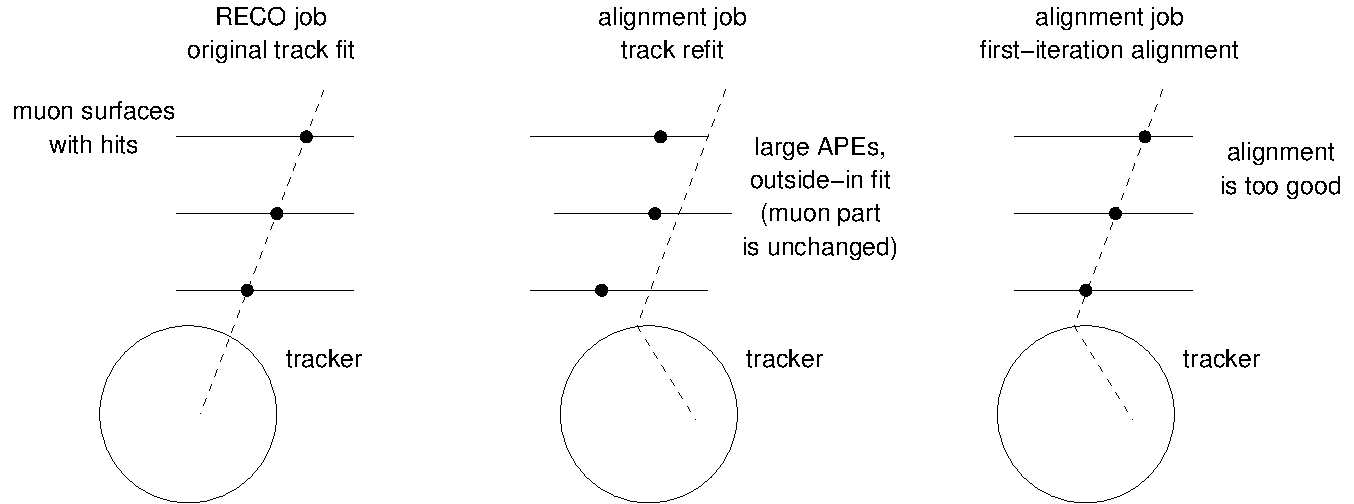
\includegraphics[width=\linewidth]{mistake.pdf}

\vfill Ideal RECO geometry creates ideally-fitted tracks.  These
should be re-fit in the alignment algorithm, but because the APEs were
large {\it and} the fit was outside-in, that part of the track was not changed.

\vfill Alignment output was too good because information about the
ideal geometry was stored in the unchanged part of the track
\end{frame}

\begin{frame}
\frametitle{How we found it with CSA07}

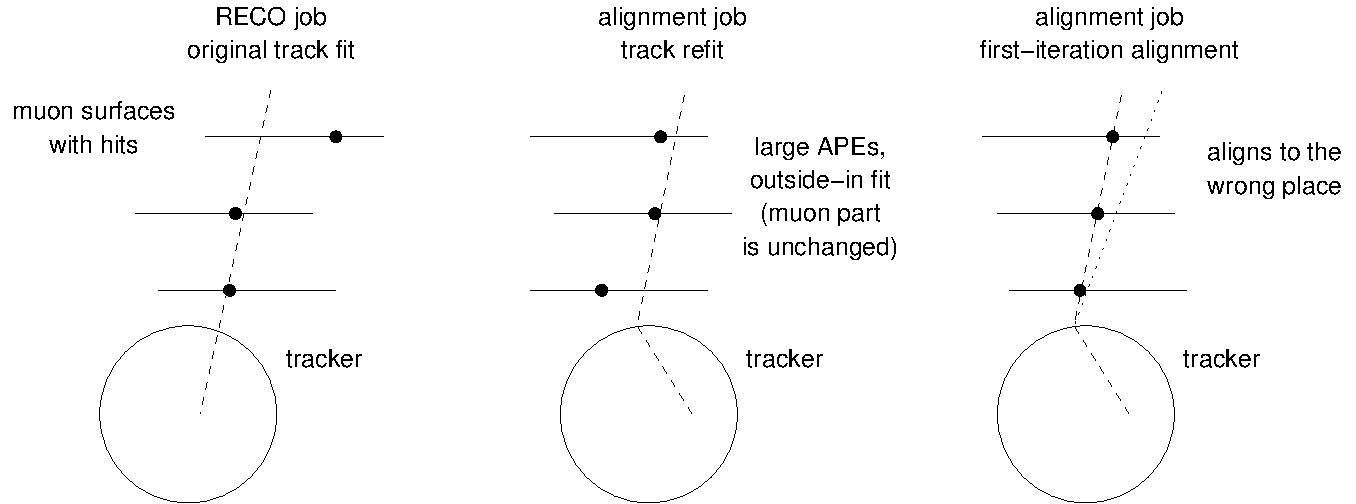
\includegraphics[width=\linewidth]{mistake2.pdf}

\vfill CSA07 event samples are misaligned at the RECO level, so we get
a non-ideal tracking seed.  The muon part of the track is again not
changed, so we incorrectly align to whatever was used in RECO.

\vfill (At first, I thought this was because a misaligned scenario was
used in simulation.)

\end{frame}

\begin{frame}
\frametitle{Verification process: to be certain that this is the problem}

We isolated the cause by reconstructing and aligning our own
$Z\to\mu\mu$ sample under every combination of CMSSW version
\begin{itemize}
\item 1\_5\_4
\item 1\_6\_4
\end{itemize}
and geometry (ideal, misaligned)
at each stage of reconstruction
\begin{itemize}
\item local RecHit reconstruction
\item muon track-fitting
\item muon id
\end{itemize}

\vfill The problem is 100\% correlated with misaligned geometry in muon
track-fitting

\end{frame}

\begin{frame}
\frametitle{Alignment quality with inside-out refitting (preliminary)}

100k events, 8 mm APEs in the muon system, 3 iterations

\begin{center}
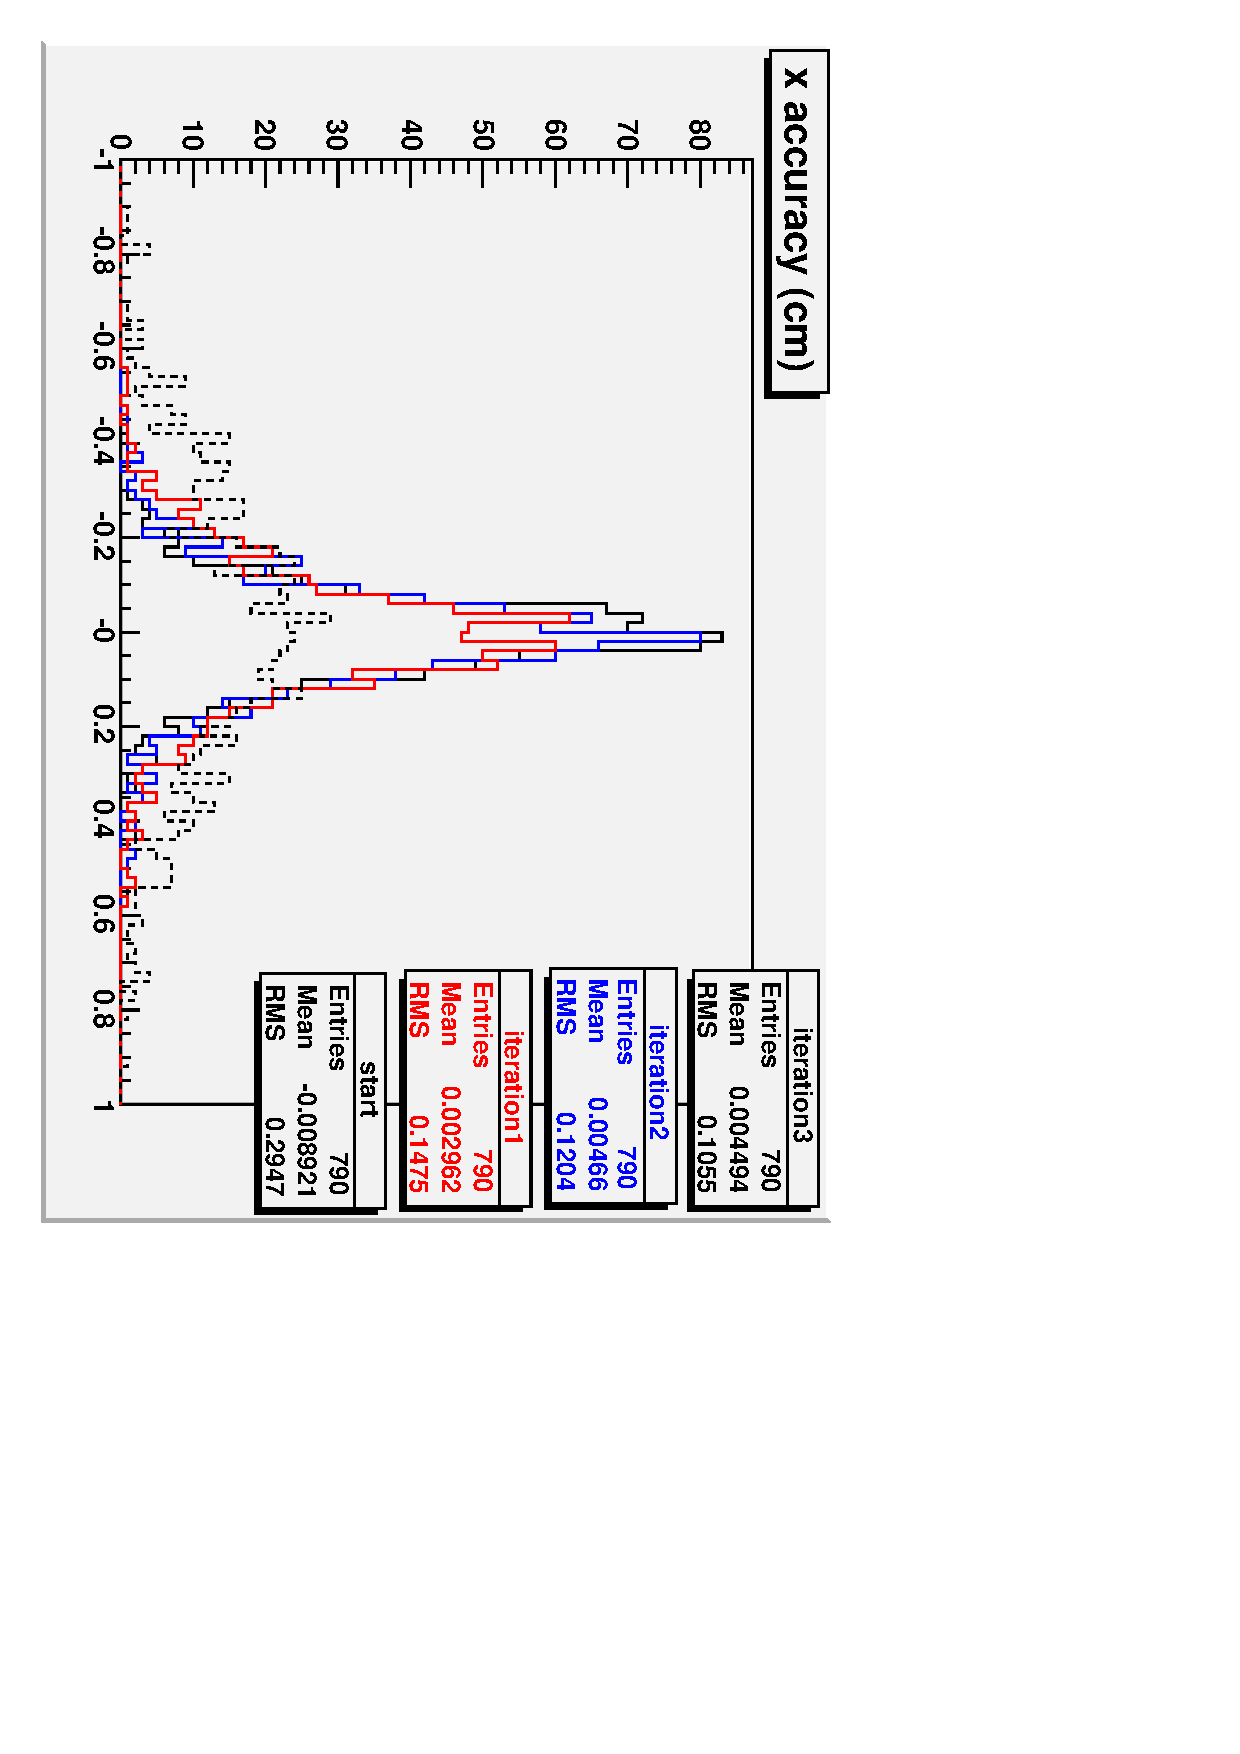
\includegraphics[height=0.6\linewidth, angle=90]{xaccuracy_3iters.pdf}
\end{center}

\vspace{-0.25 cm}
\hspace{-0.5 cm} \begin{minipage}{\linewidth}
\begin{tabular}{c c c c c}
& 1 & 2 & 3 & 4 \\\hline
Muon barrel stations & 490~$\mu$m & 680~$\mu$m & 960~$\mu$m & 1.4~mm \\
Muon endcap ME$x$/1 stations & 510~$\mu$m & 670~$\mu$m & 980~$\mu$m & 1.1~mm\\
Muon endcap ME$x$/2 stations & 830~$\mu$m & 1.2~mm & 1.5~mm & \\
\end{tabular}
\end{minipage}
\end{frame}

\begin{frame}
\frametitle{Further improvements}
\begin{itemize}
\item More iterations and an optimized descending-APE scheme (naturally)

\item Accuracy is limited by extrapolation through material: can make
better use of tracks by aligning one station at a time
\begin{enumerate}
\item Set APEs for each station to 8~mm, $\infty$, $\infty$, $\infty$
\item Align station 1
\item Set APEs for each station to 0~mm, 8~mm, $\infty$, $\infty$
\item Align station 2\ldots
\end{enumerate}

\item More resources will be required, probably tens to a few hundred CPU hours
\end{itemize}

\vfill
\hspace{-0.83 cm} \textcolor{darkblue}{\Large Conclusions}
\begin{itemize}
\item Very good news: we found this mistake in time to fix it
\item Bad news: all of our results, systematics studies, etc.\ need to be updated with a new procedure
\end{itemize}
\label{numpages}
\end{frame}

\end{document}
